\section{The Training Tool}
Here the appropriate way of using the training tool is explained in detail.

\subsection{Access}
The tool is hosted by a web page and can thus be accessed via browser.

\subsection{Uploading a CSV File in the Tool}
The user will need to feed the tool a CSV file containing properly marked values for the algorithm the user has intention of training.

This can be done by selecting the "Selezionare il file" button, which will open a window from which the user will be able to select the CSV file he has intention of uploading.

\begin{figure}[H]
\centering
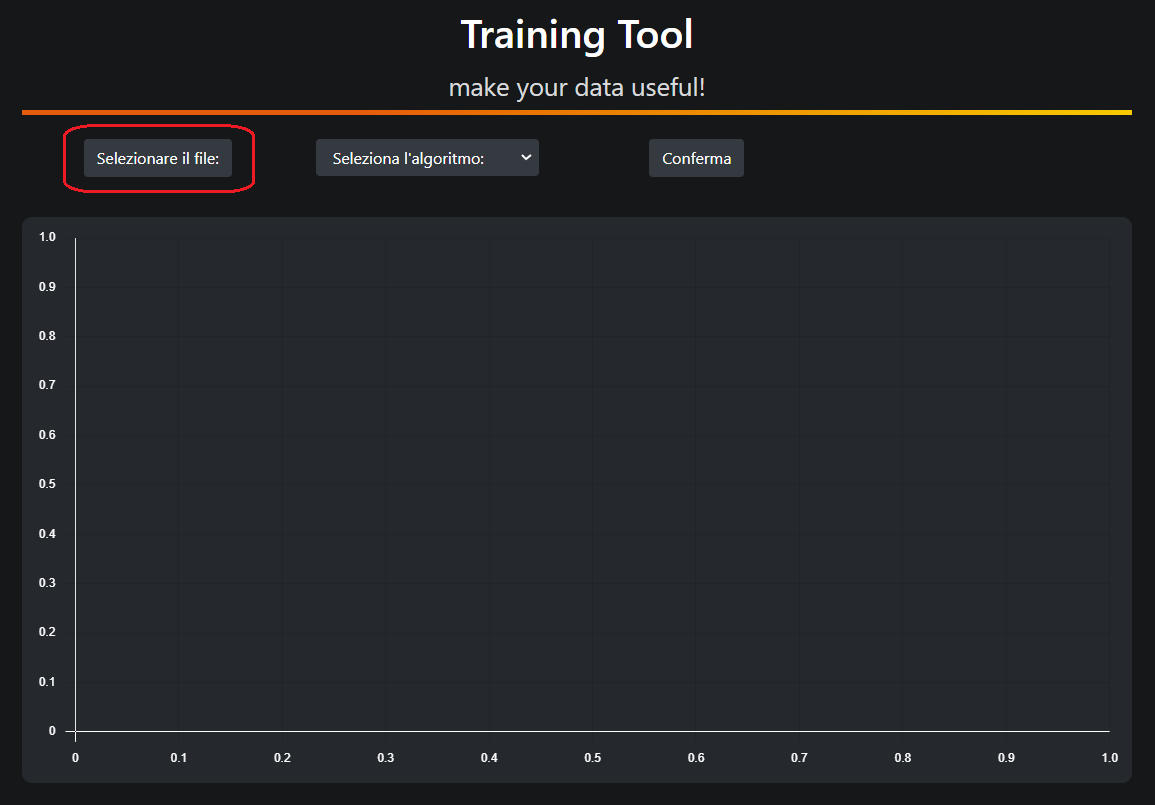
\includegraphics[scale=0.65]{img/tool/pointer_tool_1.png}
\caption{CSV-File selector}
\end{figure}
\newpage

\subsection{Selection of the Algorithm}
The user will then have to choose between training a support vector machine or a linear regression algorithm with the CSV file he has given to the tool.

To do this, the user can open a drop-down menu called "seleziona l'algoritmo" which displays the two algorithms that can be chosen, the preferred algorithm can at this point be selected.
\begin{figure}[H]
\centering
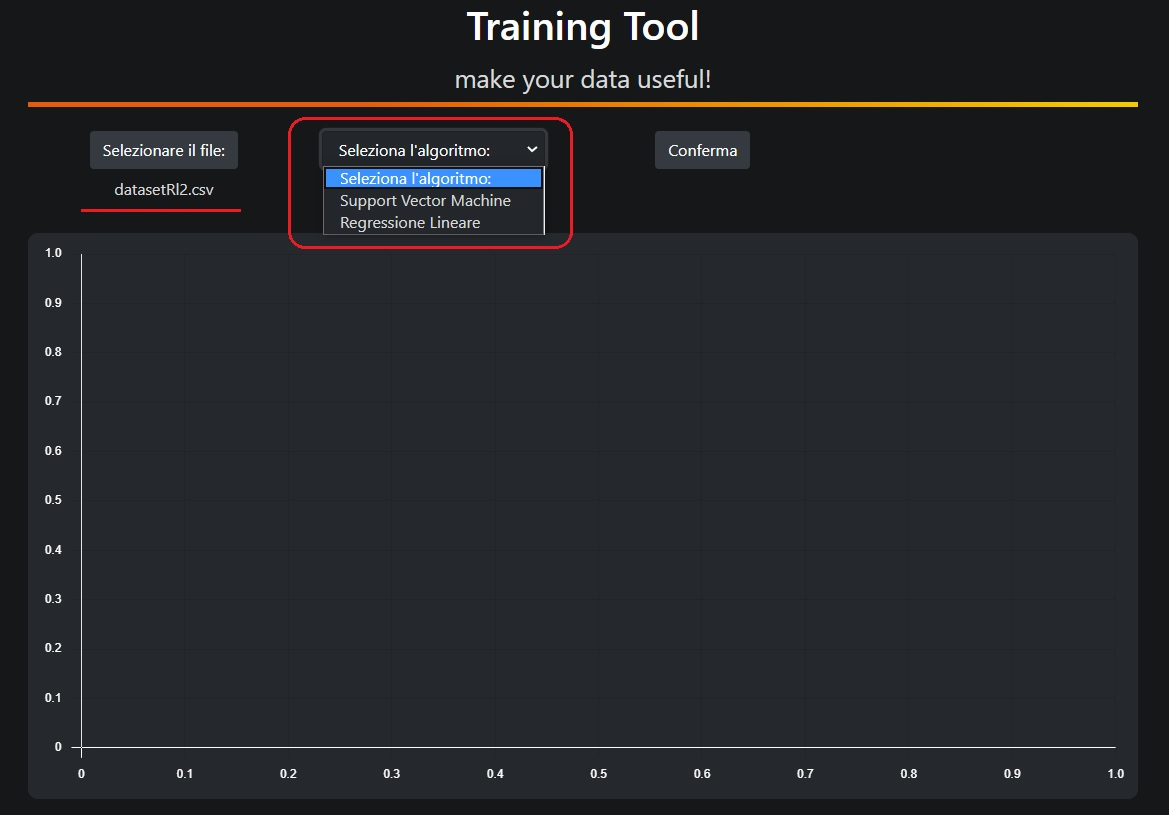
\includegraphics[scale=0.65]{img/tool/algo_selector.jpg}
\caption{Training algorithm selector}
\end{figure}
Should the user have uploaded training data incompatible with the selected algorithm, an error message will be displayed on selection of the "Conferma" button.\newline
\begin{figure}[H]
\centering

\includegraphics[scale=0.65]{img/tool/err_msg_algo.jpg}
\caption{Incompatible algorithm uploaded}
\end{figure}
\newpage
\subsection{Training Operation}
The tool will now be able to perform the training operation by simply  having the user select the “Conferma” button. The tool will now have produced a JSON file containing the values needed for use in the plug-in.
\begin{figure}[H]
\centering
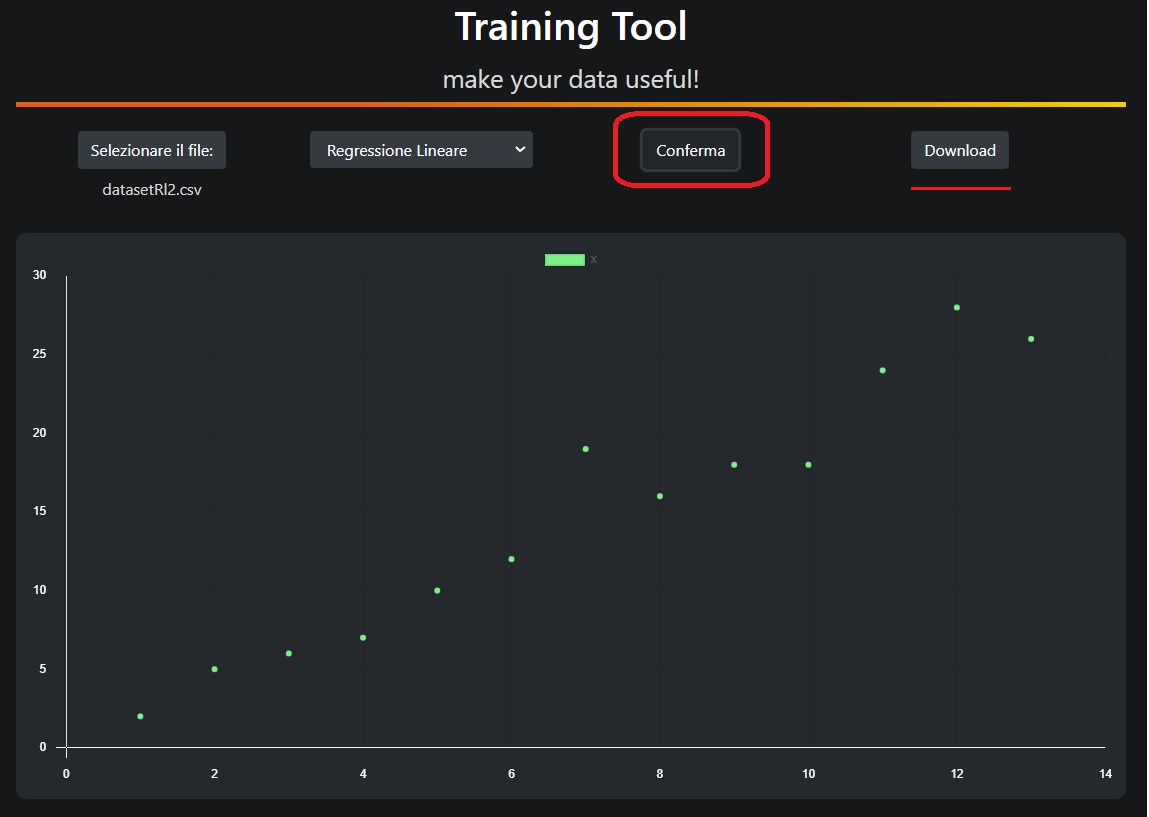
\includegraphics[scale=0.65]{img/tool/confirm.jpg}
\caption{Training operation with graphic point}
\end{figure}

A message will be displayed on selection of the "Conferma " button if the training operation is successfully completed
\newline
\begin{figure}[H]
\centering

\includegraphics[scale=0.65]{img/tool/ok_msg.jpg}
\caption{Training operation is successfully completed}
\end{figure}  

\subsection{Obtaining the JSON File}
The user can now select the “download” button, which will only appear once the training operation has ended succesfully, and receive the JSON file.
\begin{figure}[H]
\centering

\includegraphics[scale=0.65]{img/tool/ok_msg.jpg}
\caption{The "Download" button is then clickable}
\end{figure} 
